% generated by scripts/pkl_to_latex.py
% source PKL : vscan_v1_L8_Ne8_U10_t1_mode-uniform_nmin2_solver-gcg_sz0_es_restarts8_iter200_kmax4_tol1em09_V0to15_N16-2f7c06936fa2.pkl
% scan type  : vscan
% state      : ex_singlet
% requires   : \usepackage{pgfplots} \pgfplotsset{compat=1.18}
% colours match the matplotlib PDF (tab10 cycle)
\definecolor{gmeC0}{HTML}{1F77B4}
\definecolor{gmeC1}{HTML}{FF7F0E}
\definecolor{gmeC2}{HTML}{2CA02C}
\definecolor{gmeC3}{HTML}{D62728}
\definecolor{gmeC4}{HTML}{9467BD}
\definecolor{gmeC5}{HTML}{8C564B}
\definecolor{gmeC6}{HTML}{E377C2}
\definecolor{gmeC7}{HTML}{17BECF}

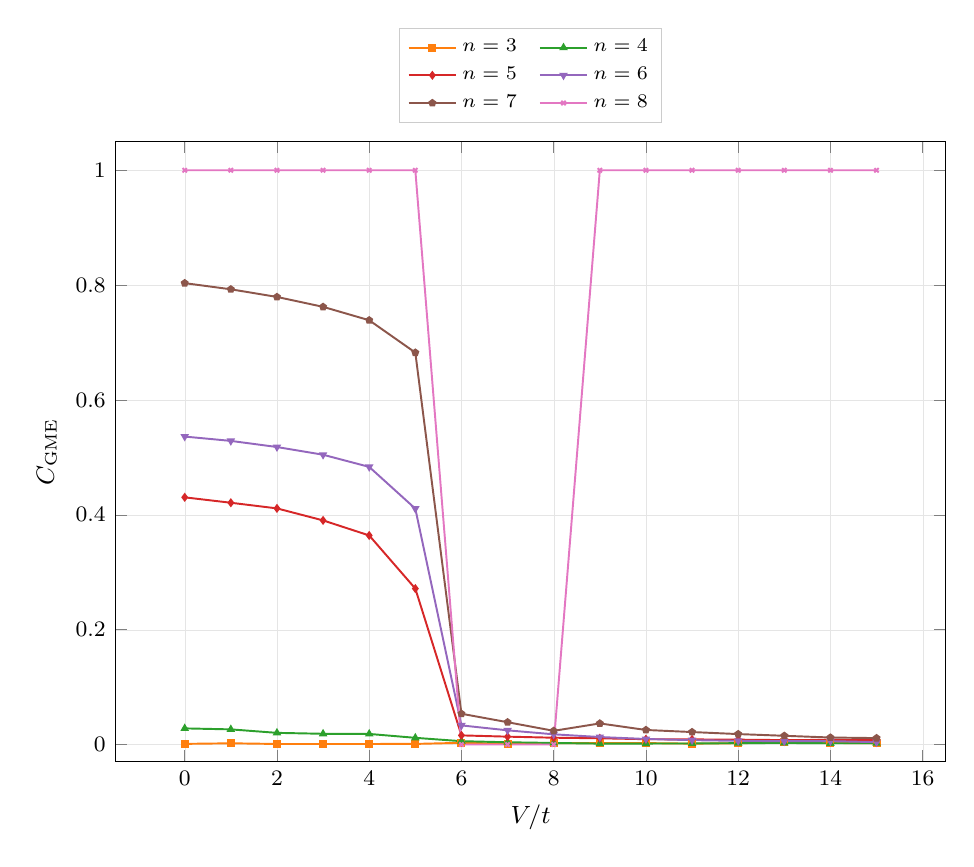
\begin{tikzpicture}
  \begin{axis}[
    width=\columnwidth,
    height=0.78\columnwidth,
    xlabel={$V/t$},
    ylabel={$C_{\mathrm{GME}}$},
    grid=both,
    grid style={line width=.1pt, draw=gray!20},
    tick label style={font=\footnotesize\rmfamily, /pgf/number format/fixed},
    label style={font=\small\rmfamily},
    scaled ticks=false,
    legend style={font=\scriptsize\rmfamily, draw=gray!40, at={(0.5,1.03)}, anchor=south, /tikz/every even column/.append style={column sep=6pt}},
    legend cell align={left},
    legend columns=2,
    ymin=-0.03,
    ymax=1.05,
  ]
    \addplot[color=gmeC1, mark=square*, mark size=1.1pt, line width=0.7pt] coordinates {
        (0,0.001114) (1,0.002115) (2,0.000955) (3,0.000906)
        (4,0.00092) (5,0.001047) (6,0.002937) (7,0.001438)
        (8,0.002496) (9,0.002515) (10,0.002467) (11,0.001535)
        (12,0.002262) (13,0.003811) (14,0.002784) (15,0.002071)
    };
    \addlegendentry{$n=3$}
    \addplot[color=gmeC2, mark=triangle*, mark size=1.1pt, line width=0.7pt] coordinates {
        (0,0.02808) (1,0.026361) (2,0.020289) (3,0.01868)
        (4,0.01842) (5,0.01165) (6,0.005797) (7,0.003933)
        (8,0.002697) (9,0.001556) (10,0.00169) (11,0.001835)
        (12,0.002367) (13,0.002733) (14,0.002154) (15,0.002217)
    };
    \addlegendentry{$n=4$}
    \addplot[color=gmeC3, mark=diamond*, mark size=1.1pt, line width=0.7pt] coordinates {
        (0,0.430438) (1,0.421014) (2,0.411191) (3,0.390284)
        (4,0.36406) (5,0.271544) (6,0.015891) (7,0.013684)
        (8,0.011842) (9,0.010855) (10,0.009255) (11,0.008899)
        (12,0.008459) (13,0.007676) (14,0.008107) (15,0.00773)
    };
    \addlegendentry{$n=5$}
    \addplot[color=gmeC4, mark=triangle*, mark size=1.1pt, mark options={rotate=180}, line width=0.7pt] coordinates {
        (0,0.536278) (1,0.528726) (2,0.518072) (3,0.504618)
        (4,0.483454) (5,0.41076) (6,0.033279) (7,0.024694)
        (8,0.017757) (9,0.013039) (10,0.009611) (11,0.007606)
        (12,0.006431) (13,0.005727) (14,0.005878) (15,0.004152)
    };
    \addlegendentry{$n=6$}
    \addplot[color=gmeC5, mark=pentagon*, mark size=1.1pt, line width=0.7pt] coordinates {
        (0,0.803455) (1,0.792734) (2,0.77942) (3,0.762191)
        (4,0.738835) (5,0.682506) (6,0.053573) (7,0.038834)
        (8,0.023845) (9,0.036722) (10,0.025329) (11,0.021708)
        (12,0.018177) (13,0.015202) (14,0.012187) (15,0.011181)
    };
    \addlegendentry{$n=7$}
    \addplot[color=gmeC6, mark=x, mark size=1.1pt, line width=0.7pt] coordinates {
        (0,1) (1,1) (2,1) (3,1)
        (4,1) (5,1) (6,0) (7,0)
        (8,0) (9,1) (10,1) (11,1)
        (12,1) (13,1) (14,1) (15,1)
    };
    \addlegendentry{$n=8$}
  \end{axis}
\end{tikzpicture}
